\documentclass[11pt,a4paper]{article} % Font size and paper type
\pagestyle{empty} % Suppress page numbers
\usepackage[left=2cm,top=2cm,right=2cm,bottom=2cm]{geometry}
\usepackage[utf8]{inputenc}
\usepackage[dvipsnames]{xcolor}
\usepackage[parfill]{parskip} % Remove paragraph indentation
\usepackage{graphicx}
\usepackage{enumitem}
\setitemize{itemsep=-5pt,leftmargin=*,label={-},topsep=-5pt}
\usepackage[colorlinks=true,urlcolor=MidnightBlue]{hyperref}

\newcommand{\hSection}[1]{
    \medskip
    \MakeUppercase{\bf #1}
    \medskip
    \hrule
}
\newcommand{\hSectionI}[2]{
    \medskip
    \MakeUppercase{\bf #1}
    \hfill
    #2
    \medskip
    \hrule
}
\newcommand{\hSubsectionA}[2]{{#1}\hfill {#2}\hspace{-1cm}}
\newcommand{\hSubsectionB}[3]{
    {#1} \hfill {#2}\hspace{-1cm}\\
    \vspace{-0.2cm} \hspace{-0.17cm}\textit{\footnotesize #3}
    \vspace{0.1cm}
}
\newcommand{\hSubsection}[2]{{#1}\hfill {#2}}
\newcommand{\hSubsectionItemize}[3]{
    {#1}\hfill {#2}\hspace{-1cm}\\
    \vspace{-0.5cm}
    \begin{itemize} \footnotesize #3 \end{itemize}
    \vspace{0.3\baselineskip}
}

\begin{document}

\begin{center}
    {\LARGE \bf VILÉM ZOUHAR} \\
    {\large \href{mailto:vilem.zouhar@gmail.com}{\color{black}{vilem.zouhar@gmail.com}}}
\end{center}

\vspace{\baselineskip}

\begin{minipage}{0.75\textwidth}
\hSection{Education}\vspace{0.2cm}
{\bf Charles University in Prague} \hfill {2017/18 - 2019/20} \\
BSc. in Computer Science \\
specialization in Computational linguistics \\
Thesis \href{https://dspace.cuni.cz/bitstream/handle/20.500.11956/119400/130284419.pdf?sequence=1&isAllowed=y}{Enabling Outbound Machine Translation}

\vspace{\baselineskip}

{\bf Saarland University\hspace{-0.1cm} +\hspace{-0.1cm} Groningen University} \hfill {2020/21 - exp. 2022/23} \\
MSc. in Language Science and Technology \\
Double degree programme \\
Thesis TBD
\end{minipage}
% 
% 
\begin{minipage}{0.25\textwidth}
    \center
    \vspace{-1cm}
    \hfill
    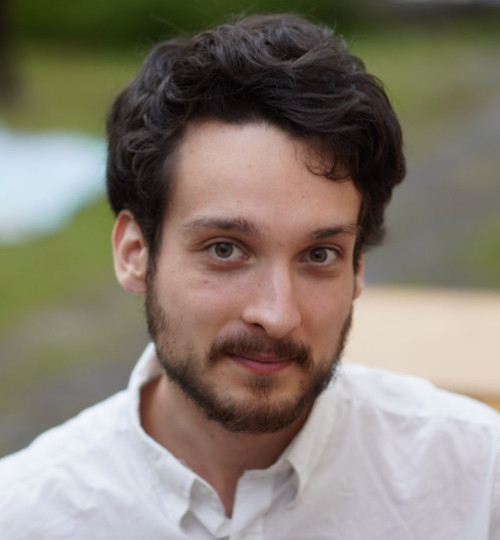
\includegraphics[width=3.5cm]{portrait.jpg}
    \vspace{-0.9cm}
\end{minipage}

\hSectionI{Selected Academic Projects and Publications}{\href{https://scholar.google.com/citations?user=2EUDwtkAAAAJ}{Google Scholar}\hspace{-1.12cm}}

\hSubsectionB
{Providing Backtranslation Improves Users Confidence in MT, Not Quality}
{NAACL 2021 accepted}
{Vilém Zouhar, Michal Novák, Matúš Žilinec, Ondřej Bojar, Mateo Obregón, Robin L. Hill,\\ Frédéric Blain, Marina Fomicheva, Lucia Specia, Lisa Yankovskaya}
\vspace{-0.11cm}

\hSubsectionB
{Leveraging Neural Machine Translation for Word Alignment}
{PBML 116 accepted}
{Vilém Zouhar, Daria Pylypenko}

\hSubsectionB
{WMT20 Document-Level Markable Error Exploration}
{\href{http://www.statmt.org/wmt20/pdf/2020.wmt-1.41.pdf}{WMT20} published}
{Vilém Zouhar, Tereza Vojtěchová, Ondřej Bojar}

\hSubsectionB
{Extending Ptakopět for MT User Interaction Experiments}
{\href{https://ufal.mff.cuni.cz/pbml/115/art-zouhar-novak.pdf}{PBML 115} published}
{Vilém Zouhar, Michal Novák}

\hSubsectionB
{Outbound Translation User Interface Ptakopet: A Pilot Study}
{\href{https://www.aclweb.org/anthology/2020.lrec-1.860.pdf}{LREC 2020} published}
{Vilém Zouhar, Ondřej Bojar}

\hSubsectionB
{A Collection of Machine Learning Excercises}
{2018/2019}
{50 pages of ML tasks in R; full version available per request (used as \href{http://ufal.mff.cuni.cz/courses/npfl054}{teaching material})}

\hSubsectionA
{Paper on machine translation evaluation}
{in writing}

\hSubsectionA
{Paper on machine translation with eyetracking}
{in writing}

\vspace{\baselineskip}
\begin{minipage}{.63\textwidth}
    \hSection{Technical Knowledge}
    \hspace{-0.3cm}
    \begin{minipage}{\textwidth}
        \vspace{0.15cm}
        \begin{tabular}{ l l}
        {\bf Programming} & JS/TS, Python, Rust, R, C/C++ \\
        {\bf Toolkits} & PyTorch, TF (basics), NLTK, Marian NMT \\
        {\bf Misc.} & Linux, Matplotlib \\
        \cr
        \end{tabular}
    \end{minipage}
\end{minipage}
\begin{minipage}{.37\textwidth}
    \hSection{Language Proficiency}
    \hspace{-0.3cm}
    \begin{minipage}{\textwidth}
        \vspace{0.15cm}
        \begin{tabular}{ l l}
        {\bf Czech} & Native \\
        {\bf English} & C1-C2\\
        {\bf German} & B2 \textit{(in development)} \\
        {\bf Polish} & A1
        \end{tabular}
    \end{minipage}
\end{minipage}

\hSection{Work Experience}
\hSubsectionItemize
{\href{https://www.lsv.uni-saarland.de/}{Spoken Language Systems} group (student research assistant)}
{2021-present}
{
    \item University of Saarland (Germany)
    \item Language modelling with external source of information
}

\hSubsectionItemize
{\href{https://teaching.lsv.uni-saarland.de/snlp/}{Statistical Natural Language Processing} class (tutor)}
{summer 2021}
{
    \item University of Saarland (Germany)
    \item Prepared \href{https://github.com/zouharvi/uds-snlp-tutorial}{class material}
}

\hSubsectionItemize
{\href{https://ufal.mff.cuni.cz}{Institute of Formal and Applied Linguistics} (student research assistant)}
{2018-present}
{
    \item Charles Univeristy (Czech Republic)
    \item Machine translation related projects
    \item \href{https://browser.mt/}{Bergamot project} (in-browser MT)
    \item Psycholinguistic project consultation
    \item Miscellaneous research tasks
}

\hSubsectionItemize
{Previo (intern software dev)}
{summer 2018}
{
    \item Development of multilayer CMS using JS, PHP, Zend and MySQL
}

\hSubsectionItemize
{BIM Project (intern software dev)}
{summer 2017}
{
    \item Development of plugins for the ArchiCAD suite with C++/Boost and C\#
}

\hSubsectionItemize
{Web development}
{2015-2017}
{
\item Participation in several commercial website projects using the PHP/JS/HTML/CSS stack
\item Brno bez vizuálního smogu, MrFox, Velab, Intimedcare 
}

\hSection{Extra-Curricular}
\hSubsectionItemize
{Academic senate}
{2018-2020}
{
\item Member of the Academic Senate at Charles University Faculty of Mathematics and Physics
}

\hSubsectionItemize
{Game Jams}
{2015-2020}
{
\item Various game jams, mostly Ludum Dare
\item Several \href{https://github.com/allemansratten}{games} programmed and presented in limited time
}

\hSubsectionItemize
{Misc. projects}
{present}
{
\item Small projects either for convenience, or as a hobby; code hosted at \href{https://github.com/zouharvi}{GitHub}
}

\hSubsectionItemize
{Kasiopea}
{2017-2019}
{
\item Organization of Kasiopea, an annual coding competition for talented highschool students
}

\end{document}

